\documentclass[12pt,letterpaper]{article}

% just for the example
\usepackage{lipsum}
% Set margins to 1.5in
\usepackage[margin=1.5in]{geometry}
\usepackage[toc,page]{appendix}

% for graphics
\usepackage{graphicx}
\graphicspath{{./figures/m1/}}

% for crimson text
\usepackage{crimson}
\usepackage[T1]{fontenc}

% setup parameter indentation
\setlength{\parindent}{0pt}
\setlength{\parskip}{6pt}

% for 1.15 spacing between text
\renewcommand{\baselinestretch}{1.15}

% For defining spacing between headers
\usepackage{titlesec}
% Level 1
\titleformat{\section}
  {\normalfont\fontsize{18}{0}\bfseries}{\thesection}{1em}{}
% Level 2
\titleformat{\subsection}
  {\normalfont\fontsize{14}{0}\bfseries}{\thesection}{1em}{}
% Level 3
\titleformat{\subsubsection}
  {\normalfont\fontsize{12}{0}\bfseries}{\thesection}{1em}{}
% Level 4
\titleformat{\paragraph}
  {\normalfont\fontsize{12}{0}\bfseries\itshape}{\theparagraph}{1em}{}
% Level 5
\titleformat{\subparagraph}
  {\normalfont\fontsize{12}{0}\itshape}{\theparagraph}{1em}{}
% Level 6
\makeatletter
\newcounter{subsubparagraph}[subparagraph]
\renewcommand\thesubsubparagraph{%
  \thesubparagraph.\@arabic\c@subsubparagraph}
\newcommand\subsubparagraph{%
  \@startsection{subsubparagraph}    % counter
    {6}                              % level
    {\parindent}                     % indent
    {12pt} % beforeskip
    {6pt}                           % afterskip
    {\normalfont\fontsize{12}{0}}}
\newcommand\l@subsubparagraph{\@dottedtocline{6}{10em}{5em}}
\newcommand{\subsubparagraphmark}[1]{}
\makeatother
\titlespacing*{\section}{0pt}{12pt}{6pt}
\titlespacing*{\subsection}{0pt}{12pt}{6pt}
\titlespacing*{\subsubsection}{0pt}{12pt}{6pt}
\titlespacing*{\paragraph}{0pt}{12pt}{6pt}
\titlespacing*{\subparagraph}{0pt}{12pt}{6pt}
\titlespacing*{\subsubparagraph}{0pt}{12pt}{6pt}

% Set caption to correct size and location
\usepackage[tableposition=top, figureposition=bottom, font=footnotesize, labelfont=bf]{caption}

% set page number location
\usepackage{fancyhdr}
\fancyhf{} % clear all header and footers
\renewcommand{\headrulewidth}{0pt} % remove the header rule
\rhead{\thepage}
\pagestyle{fancy}

% Overwrite Title
\makeatletter
\renewcommand{\maketitle}{\bgroup
   \begin{center}
   \textbf{{\fontsize{18pt}{20}\selectfont \@title}}\\
   \vspace{10pt}
   {\fontsize{12pt}{0}\selectfont \@author} 
   \end{center}
}
\makeatother

% Used for Tables and Figures
\usepackage{float}

% For using lists
\usepackage{enumitem}

% For using APA Citation format
\usepackage{apacite}

% Custom Quote
\newenvironment{myquote}[1]%
  {\list{}{\leftmargin=#1\rightmargin=#1}\item[]}%
  {\endlist}
  
% Create Abstract 
\renewenvironment{abstract}
{\vspace*{-.5in}\fontsize{12pt}{12}\begin{myquote}{.5in}
\noindent \par{\bfseries \abstractname.}}
{\medskip\noindent
\end{myquote}
}

\begin{document}

% Set Title, Author, and email
\title{Assignment M2}
\author{Snejana Shegheva \\ sshegheva3@gatech.edu}

\maketitle
\thispagestyle{fancy}

\begin{abstract}
Mapping data from one form to another for its ease-of-use is at the core of the \textit{Extract, Transform and Load} process. There exist many tools that can accomplish the task of creating and maintaining a data warehouse. However, sometimes it is advantageous to have a custom solution that allows a user to interact with the data directly during some or all of the ETL phases. In this project, we analyze an internal interface of a \textit{transform} task that prepares the data for use in a personalized recommendation system powered by Artificial Intelligence engines. 
\end{abstract}

\subsection*{Problem Space}
The data ingestion is described by the \textit{Extract, Transform and Load} (ETL) process - a cycle that converts a raw data into structured records more convenient for further Data Analysis and/or uses for Machine Learning algorithms \cite{wiki:etl}. Figure~\ref{fig::1} shows the ETL process from the Source to the Destination. The entire cycle may be completely hidden from the user (full automation of data ingestion), or a human is required to guide the components of the process to reach their desired goal. In this project we focus on the \textit{transform} task that is centered around interactions with the user to alter the original data to meet their needs. For example, a user who looks at the weather feed in Fahrenheit may choose to convert it to Celsius. 

\begin{figure}[H]
\centering
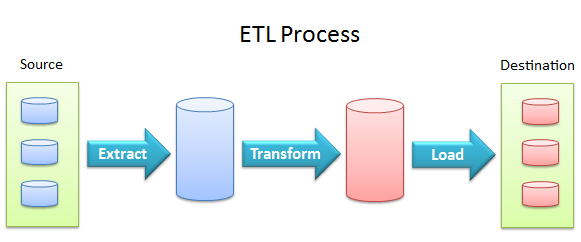
\includegraphics[width=3in, scale=.3]{ETLProcess.png}
\caption{Extract-Transform-Load Process from Data Science Central blogpost on Open Source ETL tools (https://www.datasciencecentral.com/profiles/blogs/10-open-source-etl-tools)}
\label{fig::1}
\end{figure}

To accomplish the data transformation task, a user needs access to the original data, as well as an arsenal of mapping tools suitable to the domain. Figure~\ref{fig::2} shows an existing version of an internal interface \footnote{A very rough version of a custom tool to perform user-driven ETL process.} that we will be analyzing and re-designing to improve user experience in undertaking the transformation task. 

\begin{figure}[H]
\centering
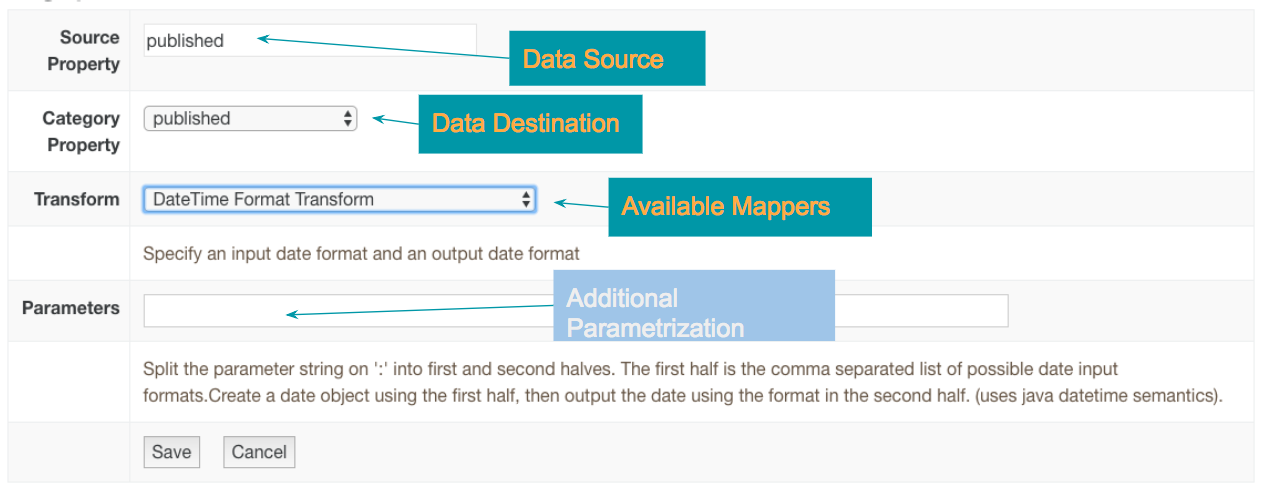
\includegraphics[width=4in, scale=.4]{NaraTransform.png}
\caption{A version of an internal interface for transforming a single data field. Here, the data source is the data from the Arxiv Library collected via ATOM API. User selects the original field, here the \textit{published} date, and wishes to transform it to a different date format.}
\label{fig::2}
\end{figure}

Our main goal is to assess all the weak areas of the existing interface in order to provide recommendations for alternative models that simplify the user interaction without assuming any pre-existing knowledge of the tool.


\subsection*{Needfinding Plan 1 - Hacks and Workarounds}
We have briefly described what the user's ultimate goal is, and how that can be broken down into sub-goals. In this section, we are going to further zoom into the user's actions for performing the task of data transformation. As our objective is to understand the weaknesses of the existing interface, as shown in Figure~\ref{fig::2}, we analyze the cases where the user breaks out of the provided interface and resorts to various hacks and workarounds to accomplish the task. A user in a Data Scientist role has a frequent need for manipulating the raw data that moves through the ETL pipeline. The main reasons why the user in that role currently changes their intended workflow and performs a subset of the actions outside of the given interface can be summarized by the following three categories: 

\begin{enumerate}
    \item \textbf{Limited functionality}. Before deciding on the transformation rules, a user needs to have a visibility on the data being transformed. In the current interface (see Figure~\ref{fig::3}), user selects the targeted data field, for example a \textit{published date}, and is given an \textit{edit} button. However, the interface does not provide enough information to make a fully informed action on the required transformation rule. Therefore, a workaround\#1:  
    \textit{Load the data in the external interface (command line, Jupyter notebooks, database queries) to explore descriptive statistics of the original field - the most frequent values,  the extreme values, the rate is missing fields, etc.}
    
    \begin{figure}[h]
    \centering
    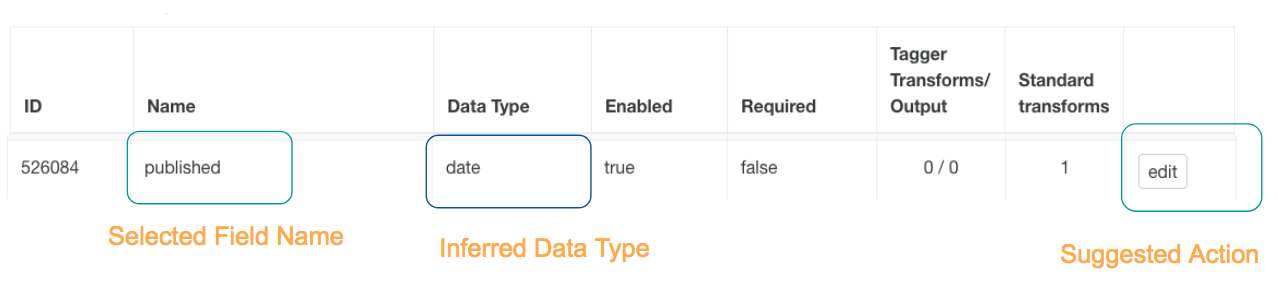
\includegraphics[width=4in, scale=.4]{DataVisibility.png}
    \caption{An example of the interface limitation to provide the user with knowledge of the present data form to enable an informed action.}
    \label{fig::3}
    \end{figure}
    
    
    \item \textbf{Poor Feature Organization}. After the user has decided on the transformation rule, the next step is to map their intentions to one of the of existing transformers. Figure~\ref{fig::4} shows that in the current interfaces the selection is given without consideration for priority or relevance of the transformation to the field being examined. Therefore, a workaround\#2:
    \textit{Browse through previously made transformations (if available) for examples and common use cases, ask colleagues for a bit of advice, or make educated guesses until the right transformer is found}
    
    \begin{figure}[h]
    \centering
    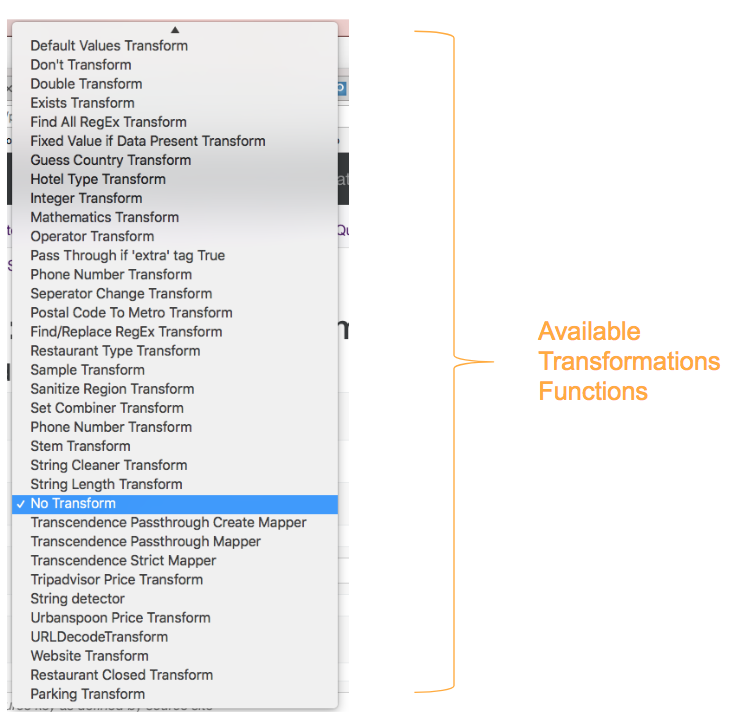
\includegraphics[width=4in, scale=.3]{Transformers.png}
    \caption{An example of the interface that displays ALL available transformation functions without priority or relevance consideration.}
    \label{fig::4}
    \end{figure}
    
    \item \textbf{Bugs in the existing functionality}. Unintended behavior in software happens all the time. The interface needs to provide accessible means to recover from a mistake by undoing an erroneous operation. A user should be comfortable exploring the interface without the fear of irreversibly corrupting the data. A good interface, therefore, should be able to guide the user from the failed state. As the current interface does not provide visibility on the original or the final data (after the applied transformation), there are no means to undo an action where transformation has the unintended effect. Workaround\#3: \textit{Modify the data via direct database access from, hopefully existing, backups.} 
    
\end{enumerate}

New type of bias: status quo:

\iffalse 

THIS IS COPIED FOR INSPIRATION: remove it!
In this needfinding method, there is little potential for bias. Possibly, we might en-counter status quo bias. Status quo bias occurs when there is an emotional preferencefor the current state of affairs. We might look at an alternate existing interface and feelthat if it is too different than what we are used to, that this would be a negative thing.To avoid this bias, we will go into the needfinding method with an open mind and theattitude that, for now, nothing is off the table.
\fi

The need-finding approach covered in this section connects the user's goals of altering a data feed to the sub-tasks of viewing the existing data, planning the transformation, and confirming the outcome. The approach of need-finding via analysis of hacks and workarounds is susceptible to \textit{observational selection bias} as we tend to notice workarounds when they impact us directly. To avoid this bias, we pair up this approach with another method that seeks to understand the pain points of a larger group of users, preferably with diverse roles.


To better understand the user's struggles with the interface, it is useful to analyze the frequencies of two kinds of errors, such as \textit{slips} and \textit{mistakes}. A mental model is a process that explains how a user is thinking about the task regarding actions and outcomes \cite{wiki:mental_model}. When a mental model matches the logic implemented by an algorithm, the user has a correct understanding of the system's functionality. In this case, the user's error can be classified as a slip vs. a mistake where the user has a wrong mental model. The approach for need-finding that focuses on error analysis broadens the spectrum of users in terms of their expertise in the given task. A novice in the field can be guided through the process of transformation by automatically matching the compatible functions to the field subjected to alterations. 

Figure~\ref{fig::5} exemplifies a hypothetical scenario where the user does not have a correct representation of the state and appropriate actions. In this example, the user attempts to transform a field that captures a person's name (\textit{author}) by applying a function that is designed to manipulate \textit{dates}. This is an incompatible operation that should not be allowed by the interface. The analysis of errors for such type outlines a \textit{need} for system's intelligence to understand the input data types and the \textit{schemata} of the available transform to reduce the space of possible matches. An improvement like can decrease the chances for user to apply incorrect action for the task at hand.   

\begin{figure}[h]
\centering
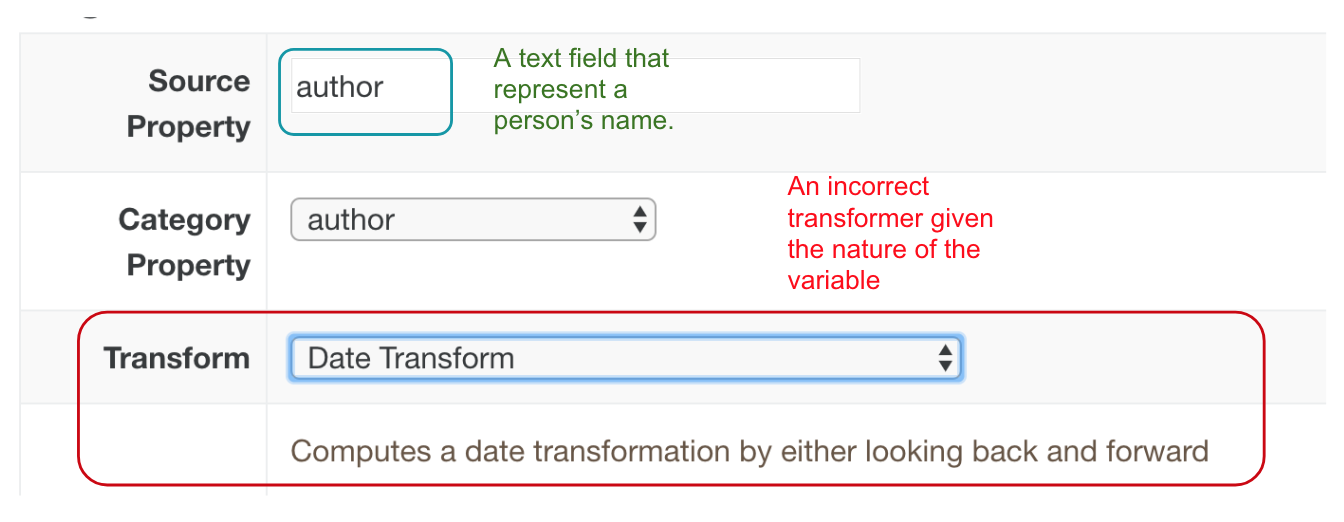
\includegraphics[width=4in, scale=.3]{mistake.png}
\caption{An example of the incorrect user action where their mental model of the underlying process is incorrect. A textual field, such as person's name cannot be computed as a date transformation.}
\label{fig::5}
\end{figure}

When a user has a correct mental model, but still makes an error due to a rushed behavior, there is an opportunity to improve the interface to reduce the chance of \textit{slippage} by altering the nature of interactions. Figure~\ref{fig::6} shows an interface that expects the user to submit a list of characters for String Cleaning. This form of interaction allows easy creation of a typo that can be avoided by modifying the underlying interaction. A change like an abstraction of special characters into a class of invalid characters for a \textit{name} field can improve users' efficiency in performing a transformation task.

\begin{figure}[h]
\centering
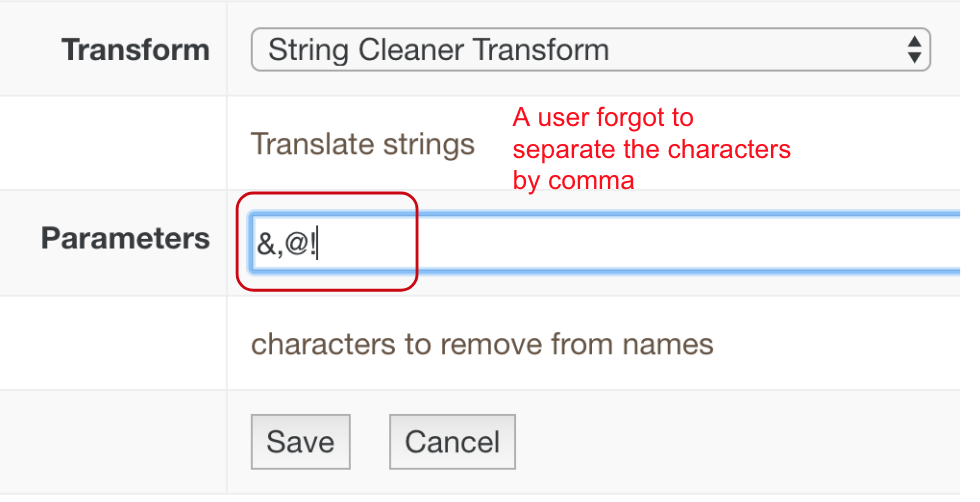
\includegraphics[width=4in, scale=.3]{slip.png}
\caption{An example of the incorrect user action where their mental model of the underlying process is correct, but user can still easily make a mistake by making a typo.}
\label{fig::6}
\end{figure}

Similarly to the approach of Hacks and Workaround, the Error analysis approach is susceptible to the \textit{observational selection} bias. In both methods, the effect of the bias can be reduced by quantitatively measuring the impact those errors have on the productivity of the end users. Metrics such as time spent troubleshooting the errors, likelihood of data corruption/loss, resources requires to re-design the specific components of the interface, etc. can help prioritize one types of errors over others.  

\subsection*{Needfinding Plan 2 - Participant Observation}
In the Participant Observation approach we experience the task ourselves and record both, the steps performed and their outcomes in order to analyze effectiveness and usability of the interface for the given task.  

\iffalse
THIS IS COPIED FOR INSPIRATION
This  section  describesthe plan  for  the needfinding  method  of participant observation.Plan for needfinding exerciseI will take up the role of a partipant observer and use the existing folder barin Piazzato filter posts by folder, as an OMSCS student enrolled in CS6750 Human Computer Interaction class. Specifically, the steps that I will follow are listed below. 1.Login to Piazza and go to CS6750 class forum.
32.Assume I am preparing for assignment P2 and hence look for folder related tothat.3.Click on folder related to assignment P24.Wait for posts in that folder to appear in the feed section.5.Browse through each postswithin the folder and search for information I need related to assignment P2. 6.Repeat step 2 to 6 with different motivations, such as searching for posts related to class participation or browsing through all folders on the bar to catch up on unread posts. I will gather data aboutwhat other activities or tasks are competing for a user’s attention when they are trying to perform the task.This relates to the context of the task from the data inventory. In addition, this needfinding method also addresses the goals of potential users, such as what outcome would a user expect from a folder bar,includinglocating the correct folder and clicking a specific folder. Lastly, I will also collect data on tasks and sub-tasks encountered when performing the filtering functionality. The data collected will be in the form of notes taken afterI participated in the task. Potential biasesOne  potential  bias  in  this  method  is  confirmation  bias.  As  I  will  be  the participation  observer, my preconceived  notions  on  the  strengthes  and weaknesses of the existing interface will affect the data I collect. The best way to limit  the  impact  is  to  forget  the  fact  that  I  am  performing  the  task  as  a participation observerfor this project, and instead pretend I am a student who genuinely need to use the folder filtering function for some purpose. Another way is to get someone who is not aware of this project to perform the task and report the results. 
\fi


\subsection*{Needfinding Plan 3 - Interviews}
Previously described two approaches on need-finding, Hacks and Workarounds, and Errors, are less prone to the social biases as they collect the outcomes of the interactions with the interface as opposed to user's responses. Those approaches, however, can be limiting in understanding the users (who they are) and their experiences in interacting with the product. Conducting User Interviews, especially the Contextual kinds, can help the designers accurately estimate the user-experience situations \cite{basics_ux_design}. The data collected from the interviews has less quantitative nature, but combining its qualitative approach with the metrics and analysis of the previous two methods leads a holistic view of the interface's strength and weaknesses.   

\textit{Contextual} interview takes place right \textit{after}, or as user \textit{is} interacting with the product. This format allows observing the main \textit{pain points} for users achieving their goal of transforming existing data. As the goals, motivations, and sub-goals are understood, the interviews must focus on the specific areas of the existing interface:

\begin{itemize}
    \item Data Presentation. What are the user benefits in being able to assess the shape and size of the data easily? Here it is important to consider that the \textit{data} is the main asset in the analyzed task)  
    \item Data Transformation. How frequently do the users need/want to manipulate the data, and alter and/or explore more complex relationships? What is the business value in incorporating the requirements of the hands-on transformation?
    \item Feedback/Recovery. What is the role of the interface in continuously providing feedback on the user's actions? What problems do the interfaces help solve, and what are the product benefits from providing a solution?
\end{itemize}

The process of collecting and analyzing the answers to the questions posed above helps avoid the common trap - \textit{you are not your user}. What the interface designer might consider as the most important feature does not necessarily match the user's needs. The need-finding research conducted via interviews connects benefits between end-user, product and business value overall. The bias of the Interview approach might arise if the group selected for the interview is susceptible to a single view of the interface and its functionality. For example, engineers may have conceptual models of the task that bias the design towards the processor model. As code implementers, they might have a pre-conceived notion on the workflow for the given task. To address this bias the interview needs to include users from other areas as well, such as business (Product Managers), Analytics (data scientists), and Infrastructure (DevOps). 

\iffalse 
THIS IS COPIED FOR INSPIRATION
The main bias I expect to encounter with the interviewis recallbias. The user may remember things differently, or have difficulty remembering during the interview. To combat this, I will need to carefully analyze the data coming from the interview and compare it with the data from theother needfinding methods. Being aware and consciousof this bias should be sufficient for combating it. 
\fi



\bibliographystyle{apacite} 
\bibliography{bibtemp}

\appendix

\section{Interview Questions}

\subsubsection*{Section 1 - Data Presentation}
When deciding to transform a property, what is the value for you in being able to see the sample of existing data for the given property? If you do not see a value on that, please explain why.  If you see a value, please provide a recommendation on what constitutes a good sample, for example, you want to see the most recent values, the most frequent values, the most extreme values, etc. If you choose to say "yes" to the value, then please justify your needs. Here, you can describe your role, and why is this important to you.  

\subsubsection*{Section 2 - Data Transformation}
How frequently the data you loaded requires additional manipulation? What are your typical scenarios for transformations? When transforming a variable, do you need access to the other variables in a single record? What is one type of transformation that you need/want the most?  

\subsubsection*{Section 3 - Feedback/Recovery}
Do you feel that the current system's feedback is adequate? For example, recall scenarios where you wanted to transform a variable, but were struggling with the interface in terms of selecting needed information (selecting a transform type, configuring the transform, etc). What is your experience at the times where the transformation you applied had an unexpected effect? Did you have enough information to understand the issue and/or recover your data and re-iterate the process?

\section{\\Interview Raw Responses}

\subsection*{Role: Senior Product Manager, Client Lead}
\subsubsection*{Question 1 - Data Presentation} 

\begin{itemize}
    \item I end up going through this process for at least half of our customers
    \item Data presentation is helpful, but only crticial when a more complicated transformation is required (e.g. regex). Typically, I will look at the data PRIOR to this screen because I need to make the decision to do the transformation before I land here. 
    \item Once on this screen, it would be helpful to see the 'would be' output before it's changed.
    \item NOTE: this screen is currently just a config, not a processing screen. A more seamless flow would be very helpful!
\end{itemize}

\subsubsection*{Question 2 - Data Transformation}
\begin{itemize}
    \item I tend to think that an Excel/CSV/DB table format is the easiest way to look at this data (horizontally, one record per row). This is the way we load data into the system initially, too, so I'm already familiar with looking at data in this format. 
    \item Probably my most frequent transforms at this point are concatenatipne (combining two or more values) or trimming/parsing/stripping from fields (e.g. removing characters)
    \item I don't do bucket transforms here, probably because I find them too difficult/not intuitive
    \item The dropdown has MANY transforms I have never used... largely because I don't know what they do. 
    \item The parameters field is applied inconsistently and isn't clear. What is supposed to go there? How do we configure these params? Better documentation needed.
    \item On my wishlist - it would be great to configure transcendence/standardization at this point too. Transcendence and tagging both feel like transforms to me.
\end{itemize}

\subsubsection*{Question 3 - Feedback/Recovery}
\begin{itemize}
    \item I think the issue here is two-fold. 1. This is just a configuration screen... It doesn't actually kick off any processing, so you could set this and never see the outcome. 2. We don't have an easy way to see the processed data until it is moved to the platform (aka production). Exposing these in a staging area would be ideal.
    \item There are additional steps required to get the data wired all the way through to 'final output' (e.g. the partner property). 
    \item Correcting errors is especially hard with our data processing tool. I believe we update a transform and reprocess to the correct values, but I'm not sure if that catches everything or if old/bad data can remain (e.g. if you mistakenly use a transform that in one case yields a value for a source entity... if you correct it, so now that new source entity has no value, does the old value go away?
\end{itemize}

\subsection*{Role: Chief Technical Officer}
\subsubsection*{Question 1 - Data Presentation}

\begin{itemize}
    \item Not using mental energy to imagine how data looks like before the transformation is very important to me; This allows to focus on the interface. Plus, imagination could be exhausting :)
\end{itemize}

\subsubsection*{Question 2 - Data Transformation}
\begin{itemize}
    \item I am involved in rapid prototyping for a variety of clients. During this phase, the data we get is very unclean, therefore I have to perform a lot of transformations.
    \item Main areas of transformations: Dictionary Mappings, Combining fields, Cleaning Up.
\end{itemize}

\subsubsection*{Question 3 - Feedback/Recovery}
\begin{itemize}
    \item \textit{Try it} functionality we currently have is a great way to provide a feedback in the form of almost interactively reshaping the data
    \item An area where I stumble is around naming for the current transforms. Name is not always representative.
\end{itemize}

\subsection*{Role: Chief UX Designer}
\subsubsection*{Question 1 - Data Presentation}

\begin{itemize}
    \item Not using mental energy to imagine how data looks like before the transformation is very important to me; This allows to focus on the interface. Plus, imagination could be exhausting :)
\end{itemize}

\subsubsection*{Question 2 - Data Transformation}
\begin{itemize}
    \item I am involved in rapid prototyping for a variety of clients. During this phase, the data we get is very unclean, therefore I have to perform a lot of transformations.
    \item Main areas of transformations: Dictionary Mappings, Combining fields, Cleaning Up.
\end{itemize}

\subsubsection*{Question 3 - Feedback/Recovery}
\begin{itemize}
    \item \textit{Try it} functionality we currently have is a great way to provide a feedback in the form of almost interactively reshaping the data
    \item An area where I stumble is around naming for the current transforms. Name is not always representative.
\end{itemize}

\end{document}
